
% Gradient Info
  
\tikzset {_d56l9pf75/.code = {\pgfsetadditionalshadetransform{ \pgftransformshift{\pgfpoint{0 bp } { 0 bp }  }  \pgftransformrotate{-146 }  \pgftransformscale{2 }  }}}
\pgfdeclarehorizontalshading{_9togdt637}{150bp}{rgb(0bp)=(1,1,1);
rgb(56.84058598109654bp)=(1,1,1);
rgb(59.8930413382394bp)=(0.61,0.61,0.61);
rgb(62.5bp)=(0.29,0.29,0.29);
rgb(100bp)=(0.29,0.29,0.29)}

% Gradient Info
  
\tikzset {_jbj0scktb/.code = {\pgfsetadditionalshadetransform{ \pgftransformshift{\pgfpoint{0 bp } { 0 bp }  }  \pgftransformrotate{-129 }  \pgftransformscale{2 }  }}}
\pgfdeclarehorizontalshading{_gxn22itp6}{150bp}{rgb(0bp)=(0.29,0.29,0.29);
rgb(37.5bp)=(0.29,0.29,0.29);
rgb(43.7797600882394bp)=(1,1,1);
rgb(100bp)=(1,1,1)}
\tikzset{every picture/.style={line width=0.75pt}} %set default line width to 0.75pt        

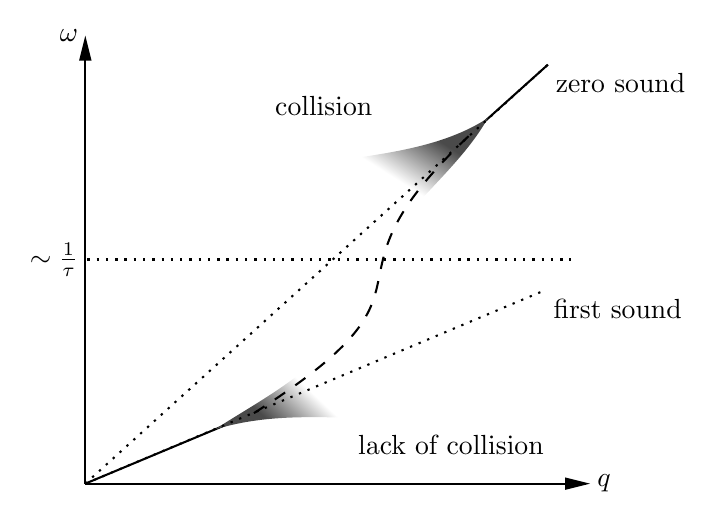
\begin{tikzpicture}[x=0.75pt,y=0.75pt,yscale=-1,xscale=1]
%uncomment if require: \path (0,300); %set diagram left start at 0, and has height of 300

%Straight Lines [id:da6006990507896193] 
\draw    (257.92,94.17) -- (325.92,33.1) ;
%Straight Lines [id:da8463599501793553] 
\draw    (103,235) -- (344.17,235) ;
\draw [shift={(346.17,235)}, rotate = 180] [fill={rgb, 255:red, 0; green, 0; blue, 0 }  ][line width=0.08]  [draw opacity=0] (12,-3) -- (0,0) -- (12,3) -- cycle    ;
%Straight Lines [id:da2275445831732943] 
\draw    (103,235) -- (103,21.19) ;
\draw [shift={(103,19.19)}, rotate = 90] [fill={rgb, 255:red, 0; green, 0; blue, 0 }  ][line width=0.08]  [draw opacity=0] (12,-3) -- (0,0) -- (12,3) -- cycle    ;
%Straight Lines [id:da6099852885108679] 
\draw    (103,235) -- (184.26,201.02) ;
%Shape: Polygon Curved [id:ds3933722880021524] 
\draw  [draw opacity=0][shading=_9togdt637,_d56l9pf75] (294.51,202.92) .. controls (242.83,207.29) and (203.28,197.08) .. (165.26,208.96) .. controls (197.68,188.2) and (225.06,176.75) .. (250.35,126.15) .. controls (261.8,137.72) and (295.13,166.87) .. (294.51,202.92) -- cycle ;
%Straight Lines [id:da7618060721275304] 
\draw  [dash pattern={on 0.84pt off 2.51pt}]  (103,235) -- (325.17,141.52) ;
%Shape: Polygon Curved [id:ds9419710356804576] 
\draw  [draw opacity=0][shading=_gxn22itp6,_jbj0scktb] (171.32,89.99) .. controls (221.15,75.65) and (263.94,80.05) .. (296.92,58.92) .. controls (278.92,90.85) and (239.92,111.85) .. (229.57,156.7) .. controls (216.08,147.58) and (177.72,125.47) .. (171.32,89.99) -- cycle ;
%Straight Lines [id:da4615538031472426] 
\draw  [dash pattern={on 0.84pt off 2.51pt}]  (103,235) -- (326.17,32.85) ;
%Curve Lines [id:da7468246422953644] 
\draw  [dash pattern={on 4.5pt off 4.5pt}]  (184.26,201.02) .. controls (286.17,136.19) and (206.17,142.19) .. (291.92,63.64) ;
%Straight Lines [id:da9243960083758465] 
\draw  [dash pattern={on 0.84pt off 2.51pt}]  (104,127) -- (337.17,127) ;

% Text Node
\draw (328.17,35.85) node [anchor=north west][inner sep=0.75pt]   [align=left] {zero sound};
% Text Node
\draw (327.17,144.52) node [anchor=north west][inner sep=0.75pt]   [align=left] {first sound};
% Text Node
\draw (348.17,235) node [anchor=west] [inner sep=0.75pt]    {$q$};
% Text Node
\draw (101,19.19) node [anchor=east] [inner sep=0.75pt]    {$\omega $};
% Text Node
\draw (193,47) node [anchor=north west][inner sep=0.75pt]   [align=left] {collision};
% Text Node
\draw (233,210) node [anchor=north west][inner sep=0.75pt]   [align=left] {lack of collision};
% Text Node
\draw (101,127.09) node [anchor=east] [inner sep=0.75pt]    {$\sim \frac{1}{\tau }$};


\end{tikzpicture}
